\documentclass{standalone}
\usepackage{tikz}
\usepackage{tkz-graph}
\usepackage{tkz-berge}

\begin{document}

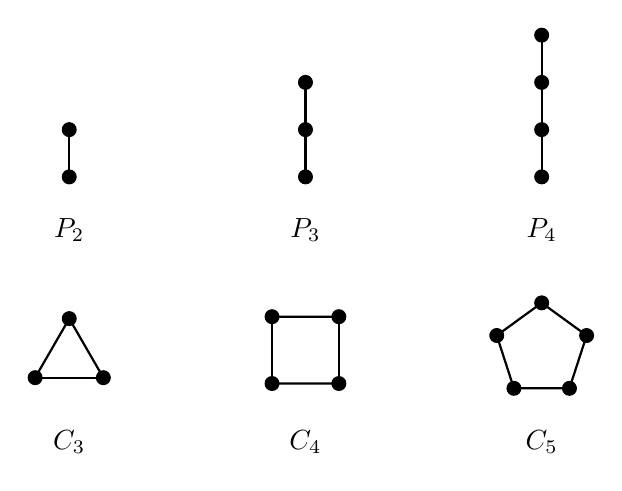
\begin{tikzpicture}
  \GraphInit[vstyle=Simple]
  \tikzset{VertexStyle/.style = {
  shape = circle,
  fill = black,
  inner sep = 0pt,
  outer sep = 0pt,
  minimum size = 5pt,
  draw}}
  \SetVertexMath
  \begin{scope}[yshift=2.2cm, rotate=90]
    \grPath[RA=0.6]{2}
  \end{scope}
  \begin{scope}[yshift=2.2cm, xshift=3cm, rotate=90]
    \grPath[RA=0.6]{3}
  \end{scope}
  \begin{scope}[yshift=2.2cm, xshift=6cm, rotate=90]
    \grPath[RA=0.6]{4}
  \end{scope}
  \begin{scope}[yshift=-0.1cm, rotate=90+((360/3)*3)]
    \grCycle[RA=0.5]{3}
  \end{scope}
  \begin{scope}[yshift=0cm, xshift=3cm, rotate=45]
    \grCycle[RA=0.6]{4}
  \end{scope}
  \begin{scope}[yshift=0cm, xshift=6cm, rotate=90+((360/5)*3)]
    \grCycle[RA=0.6]{5}
  \end{scope}
  \draw (0, 1.8) node [below]{$P_2$};
  \draw (3, 1.8) node [below]{$P_3$};
  \draw (6, 1.8) node [below]{$P_4$};
  \draw (0,-0.9) node [below]{$C_3$};
  \draw (3,-0.9) node [below]{$C_4$};
  \draw (6,-0.9) node [below]{$C_5$};
\end{tikzpicture}

\end{document}
